\documentclass[a4paper, fleqn]{article}

\usepackage{amsmath}
\usepackage{enumitem}
\usepackage{graphicx}

\begin{document}

\title{Capstone I - Journal 02 \\ Project 61 $\cdot$  Steelcase \\ Reduction of Logistics and Packaging Costs}
\author{Basil R. Yap}
\date{2018 February 23}
\maketitle

\section{Summary}

Based on my previous plans for the project, I had predicted that we would progressed a significant deal since the first few weeks of the project. Transitioning from initial logistics to the preliminary stages of data analysis and product design, partially broken down by week as follows:\begin{itemize}
\item \textbf{Week 3:} Exploratory analysis
\item \textbf{Week 4:} Data cleaning
\item \textbf{Week 5:} 1st Model creation
\end{itemize}
Sadly, due to circumstance, I was not able to meet the goals set up by the timeline. There were many aspects of the project I did not foresee, which I believe can be taken into account in future engagements with the industry partner and other projects.  \\
\vspace{1pt}\\
Despite the change in plans, I believe the productivity and abilities of the team and I were not lacking. But rather, considering having not worked on a project with such magnitude in scope and length of time, there were tasks and steps which I did not account for when planning ahead. The actual work breakdown is represented as:\begin{itemize}
\item \textbf{Week 3:} Exploratory analysis
\item \textbf{Week 4:} Evaluation of project scope
\item \textbf{Week 5:} Negotiation and readjustment of project scope
\end{itemize}
Based on limitations on time and data, the emphasis shifted to the project scope itself. Usually in other projects, this phase of the project is often overlooked due to a strict definition of the problem and the absence of design thinking involved.

\section{Problems Encountered}

Upon receiving the data and discussing at length with the industry partners, there were a few major problems my team and I encountered along the way. Many of which can be classified as follows:\begin{itemize}
\item \textbf{Lack of Representation of the system in the data}\\
The data provided was able to shed a shallow light on the inner workings of Steelcase Malaysia, but not enough to provided a detailed enough understanding of the overall system as to model it in professional manner. The data files were disjointed from one data file to another, with little connection between any two files. This created gaps in our knowledge and workings of the system, making a data driven approach very difficult.\\
\vspace{1pt}\\
From a systems perspective, it is very difficult to gather a complete view of the system, making it very difficult to account for all costs and variables in the supply chain in an accurate and meticulous manner.
\item \textbf{Incompleteness of financial and logistic data}\\
The availability of financial and inventory data were not given to us and among the data provided, any and all mention of finance related entries were censored or redacted. When requested for more finance related data, our industry partner insisted we should focus on the shipment data given if possible. Furthermore, only one year of useful outbound shipment was given, with no indication of the contents of each shipment.\\
\vspace{1pt}\\
The presence of financial and logistic is essential if we want to tackle the problem from a supply chain perspective. The presence of a financial metric allows us to compare and justify any proposals we make to our industry partners. The presence of complete logistic data is equally important, as without information about the contents of each cargo or a wider sample size of shipment data, the proposals provided akin to educated guesswork with little to no statistical evidence to support our claims.
\item \textbf{Feasibility of Initial problem scope}\\
Based on the data given to us and the advice given to us by our industry partners, the initial scope of our project no longer encapsulates our project well enough for us to use them moving forward. The initial scope was consisted of two distinct parts, supply chain optimization and packaging product design. The current direction consists mainly of packaging product design and load-space optimization, which differs quite significantly in practice.\\
\vspace{1pt}\\
The scope of the problem helps us determine the overall direction of the project and helps ensure a consensus among all stakeholders involved. If the problem scope is not set properly at the start of the project, a misalignment of expectations might occur at the later stages of the project, affecting the overall perception and performance of the project. This is why I believe it is the central focus of the First Review.  
\end{itemize}

\section{Actions Taken}

In sequential order, my team and I underwent the following tasks over the span of the last three weeks:\begin{enumerate}
\item \textbf{Exploratory Analysis of Data}\\
Taking note of the structure of each dataset/data file, I documented the contents and took note of the overall utility of each document. This allowed for the identification of documents with elements that required further clarification from our industry partners and identification of missing information that is needed to link the documents together.
\item \textbf{Clarification of Data}\\
With the information gleamed from the exploratory analysis, I liaised with the industry partners in order to clarify and rectify the discrepancies in the documents. This task also helped furnish my team and I with a better understanding of the expectations and priorities of Steelcase Malaysia.
\item \textbf{Reevaluation of Project Scope}\\
Taking into account the information and resources available, my team and I discussed about the extent of the scope of the project and management of the expectations of all the stakeholders. This task also coincides with my team's preparation for our first midterm review. I helped steer the conversation in order to solidify a feasible and tangible short term and long term goal for my team.
\end{enumerate}

\section{Insights Obtained}

\textit{Note: }The segment \textit{"Clarification of Data"} has been broken up and incorporated into the other two points. The two contributing points being, the clarification of provided data and the reevaluation of the project scope as suggested by the industry partner.
\vspace{1pt}\\
Upon observing the data, I documented the details of the files and my comments as follows:
\begin{center}
\begin{tabular}{| p{0.2\linewidth} | p{0.4\textwidth} | p{0.4\textwidth} |}
\hline
File name & Notable info & Comments\\
\hline
packaging specification and distribution guidelines & \begin{itemize}
\item Packaging test requirements 
\item List of approved materials 
\item Graphic design template  
\end{itemize} & \begin{itemize}
\item reference doc 
\item packaging
\end{itemize}\\
\hline
SMM Products Mar 2018 & \begin{itemize}
\item images of assembled products
\end{itemize}  & \begin{itemize}
\item product
\item not very informative
\item requires images of product in package
\item requires packaging instructions
\item requires product component breakdown 
\end{itemize}\\
\hline
Container utilization & \begin{itemize}
\item relative volume of exports between products
\item load-space efficiency of each product
\end{itemize}  & \begin{itemize}
\item load
\item data file
\end{itemize}\\
\hline
Shipments (inbound) & \begin{itemize}
\item -
\end{itemize}  & \begin{itemize}
\item not very useful as Steelcase Malaysia has not much control over inbound shipments
\end{itemize}\\
\hline
Shipments (outbound) & \begin{itemize}
\item seasonal frequency of exports
\item cost of shipment
\item size and weight of shipment
\end{itemize}  & \begin{itemize}
\item shipment
\item data file
\item 1 year of data (insufficient)
\end{itemize}\\
\hline
\end{tabular}
\end{center}
\begin{center}
\begin{tabular}{| p{0.2\linewidth} | p{0.4\textwidth} | p{0.4\textwidth} |}
\hline
File name & Notable info & Comments\\
\hline
Mechanism packaging & \begin{itemize}
\item images of packaged components
\item number of parts per package
\end{itemize}  & \begin{itemize}
\item packaging
\item informative but not detailed
\end{itemize}\\
\hline
Packaging cost & \begin{itemize}
\item packaging cost per product
\item volume per product
\end{itemize}  & \begin{itemize}
\item packaging
\item data file
\end{itemize}\\
\hline
Loading report & \begin{itemize}
\item container utilization per country
\end{itemize}  & \begin{itemize}
\item load
\item data file
\end{itemize}\\
\hline
\end{tabular}
\end{center}
With this information, I mapped out the potential metrics we had stipulated at the first meeting and added the information required by each metric. This allowed me to brainstorm about potential gaps in information that would prevent the project from creating meaningful results.\\
\begin{figure}[h!]
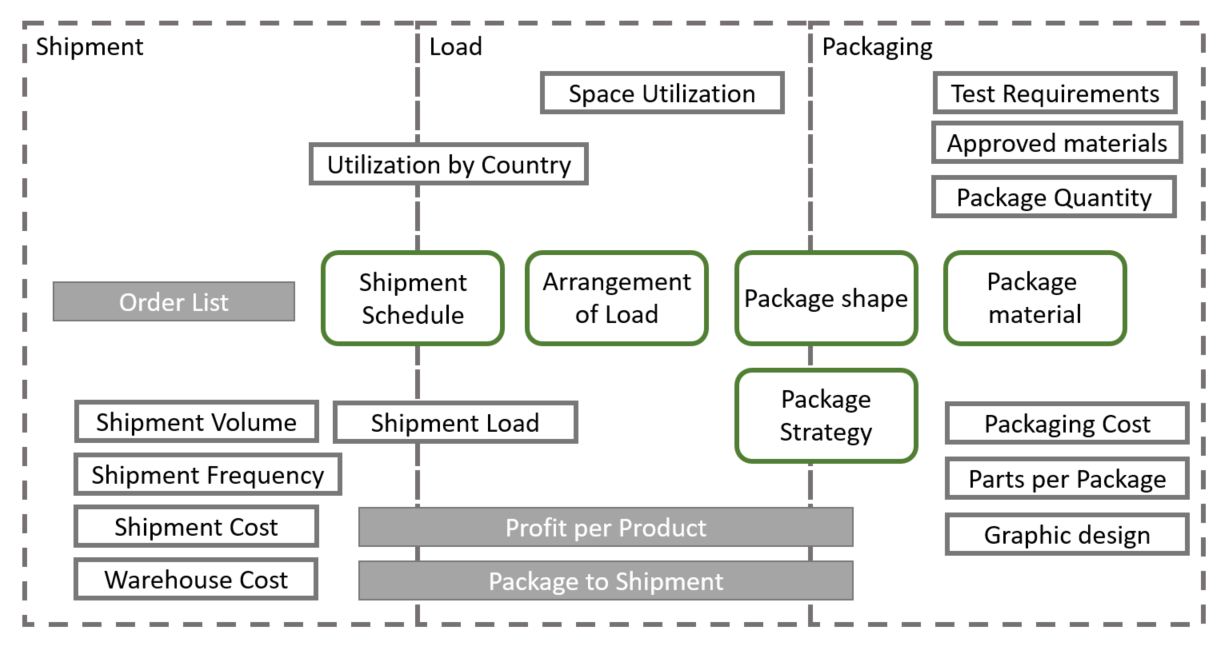
\includegraphics[width=\linewidth]{./assets/201802260436.PNG}
\caption{Map of Design Space of Project}
\label{figure:image1}
\end{figure}
It can be observed that a few essential data required for shipment scheduling (i.e. supply chain optimization) has not been provided. Therefore, our problem scope should be narrowed to load and packaging optimization.
\section{Timeline}

The my personal timeline for next three weeks are as follows:
\begin{itemize}
\item \textbf{[Preparation] Week 6:}    \begin{enumerate}
\item Complete Review I
\item Prepare questions for Site Visit
\end{enumerate}
\item \textbf{Week 7:}    \begin{enumerate}
\item Site Visit
\item Acquire more data and clean data (If applicable)
\end{enumerate}
\item \textbf{Week 8:}     \begin{enumerate}
\item Attempt to model load optimization
\item Analyze outbound shipment trends (preliminary)
\item Continue Cleaning data (If applicable)
\end{enumerate}
\item \textbf{Week 9:}    \begin{enumerate}
\item Formulate load optimization problem in AMPL
\item Improve outbound shipment trend estimation (If applicable)
\end{enumerate}
\end{itemize}

\end{document}